\documentclass[a4paper]{report}
\usepackage{hyperref}
\usepackage{lastpage}
\usepackage{fancyhdr}
\usepackage{lineno}
\usepackage{listings}
\usepackage{german}
\usepackage[utf8]{inputenc}
\usepackage{amssymb}
\usepackage{graphicx}
\usepackage{pgf-umlsd-0.7/pgf-umlsd}
\usepackage{tikz}
\usetikzlibrary{shapes,arrows}
\usepackage[final]{pdfpages}
%\newcommand{\genasso}[2]{\begin{minipage}{0.7\textwidth}\begin{normalsize}\begin{flushleft}\textbf{{#1}}\end{flushleft}\end{normalsize}\vspace{-1cm}\begin{flushleft}\begin{small}{#2}\end{small}\end{flushleft}\end{minipage}\\\vspace{0.2cm}}
\pagenumbering{arabic}

\pagestyle{fancy} 
\newcommand{\frontmatter}{\clearpage \cfoot{\thepage\ }
\setcounter{page}{1}
\pagenumbering{Roman}}
\newcommand{\mainmatter}{\clearpage \lhead{\myAuth} \rhead{\myDate} \cfoot{} \rfoot{\thepage\ of \pageref{LastPage}}
\setcounter{page}{1}
\pagenumbering{arabic}}
\newcommand{\backmatter}{\clearpage \rfoot{\thepage\ }
\setcounter{page}{1}
\pagenumbering{alph}}


\newcommand{\makemytitlepage}{\begin{titlepage}
    \begin{center}
        \vspace*{0.8cm}
        
        \Huge
        \textbf{\myTitle}
        
        \vspace{1.5cm}
        
        \Large
        \myAuthor

        \vspace{1.8cm}

        %\begin{large}\textbf{Abstract:} \myAbstract \end{large}
        
\includegraphics[width=6cm]{./IM.jpg}  
        
        \vfill
        
        \huge
        \myAsso
        
        \vspace{1.3cm}
        
        \Large

        %\myDate
        \today
        
    \end{center}
\end{titlepage}}
\newcommand{\myAuth}{Team: *Iron Man*\\B. Pohl, K. Trogant, R. Enseleit, D. Hebecker}
\newcommand{\myAuthor}{Birgit Pohl 574353 (MO. 9-11)\\Kevin Trogant 572451 (Mo. 15-17)\\Ronja Enseleit 572404 (Mo. 15-17)\\Dustin Hebecker 571271 (MO. 9-11)}
\newcommand{\myAsso}{Group: *Iron Man*}
\newcommand{\myDate}{\today}

%%%%%%%%%%%%%%%%%%%%%%%%%%%%%%%%
%%Change Title !!!!!!!!!!!!!!!!!
%%%%%%%%%%%%%%%%%%%%%%%%%%%%%%%%
\newcommand{\myTitle}{Exercise Sheet B}

\begin{document}
\frontmatter
\makemytitlepage
\mainmatter

%%%%%%%%%%%%%%%%%%%%%%%%%%%%%%%%%%%%%%%%%%%%%%%%%%%%%%%%%%
%% Only modify below here  and change myTitle!!!!!!!!!!!!!
%%%%%%%%%%%%%%%%%%%%%%%%%%%%%%%%%%%%%%%%%%%%%%%%%%%%%%%%%%
\section*{Aufgabe 1}
\begin{center}
    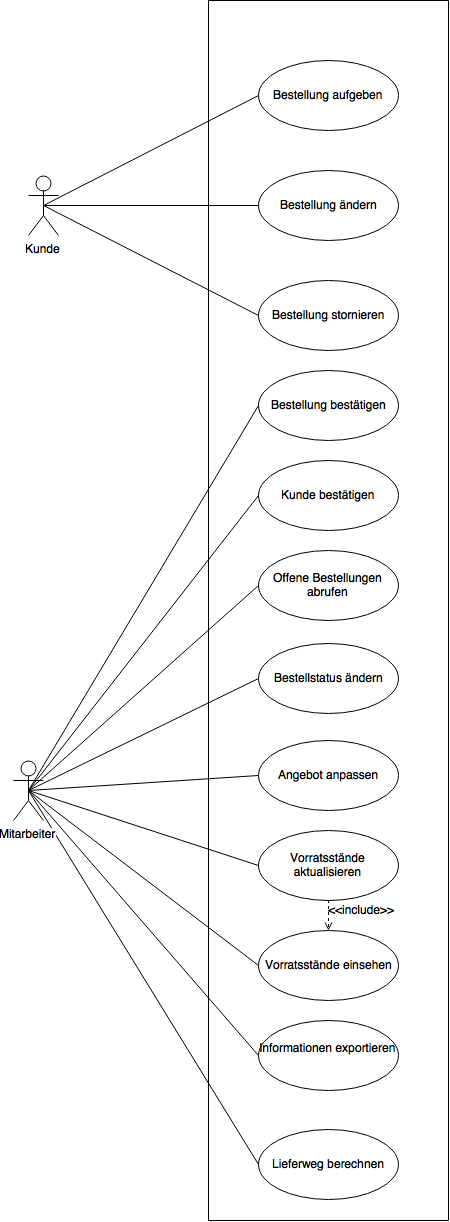
\includegraphics[width=7cm]{use_cases.png}
\end{center}

\subsection*{Textuelle Beschreibungen}
\subsubsection*{Bestellung aufgeben}
\begin{itemize}
    \item \textbf{Kurzbeschreibung:} Kunde gibt eine Bestellung aus vorher ausgewählten Gerichten auf.
    \item \textbf{Akteure:} Kunde
    \item \textbf{Vorbedingungen:} Kunde hat noch keine Bestellung aufgegeben.
    \item \textbf{Beschreibung des Ablaufs:}
        \begin{enumerate}
            \item Prüfe ob der Kunde zu einer Bestellung berechtigt ist (Kunde nicht gespeert, Lieferadresse nicht zu weit weg, ...)
            \item Wenn ja, trage die Bestellung als \textit{Neu} ins System ein und gib eine entsprechende Meldung aus
            \item Wenn nein, gib eine entsprechende Fehlermeldung aus
        \end{enumerate}
    \item \textbf{Nachbedingungen Erfolg:} Die Bestellung wird ins System eingetragen
    \item \textbf{Nachbedingungen Fehlschlag:} Eine Fehlermeldung wird angezeigt
\end{itemize}
%
\subsubsection*{Bestellung ändern}
\begin{itemize}
    \item \textbf{Kurzbeschreibung:} Kunde ändert eine vorher aufgegebene Bestellung
    \item \textbf{Akteure:} Kunde
    \item \textbf{Vorbedingungen:} Die Bestellung existiert und befindet sich im Zustand \textit{Neu} oder \textit{Backend}
    \item \textbf{Beschreibung des Ablaufs:}
        \begin{enumerate}
            \item Prüfe ob die Bestellung existiert und sich im Zustand Neu befindet. Falls die Änderung nur aus dem Hinzufügen neuer Pizzen besteht, kann die Bestellung auch im Zustand Backend sein.
            \item Wenn ja, führe die gewünschten Änderungen durch und gib eine Benachrichtigung aus.
            \item Wenn nein, gib eine entsprechende Fehlermeldung aus
        \end{enumerate}
    \item \textbf{Nachbedingungen Erfolg:} Die Bestellung wurde abgeändert
    \item \textbf{Nachbedingungen Fehlschlag:} Eine Fehlermeldung wird angezeigt
\end{itemize}
%
\subsubsection*{Bestellung stornieren}
\begin{itemize}
    \item \textbf{Kurzbeschreibung:} Kunde storniert eine Bestellung
    \item \textbf{Akteure:} Kunde
    \item \textbf{Vorbedingungen:} Die Bestellung existiert und befindet sich im Zustand \textit{Neu}.
    \item \textbf{Beschreibung des Ablaufs:}
        \begin{enumerate}
            \item Prüfe ob die Bestellung existiert und sich im Zustand \textit{Neu} befindet.
            \item Wenn ja, ändere den Zustand der Bestellung auf \textit{Abgebrochen} und gib eine entsprechende Meldung aus. 
            \item Wenn nein, gib eine entsprechende Fehlermeldung aus
        \end{enumerate}
    \item \textbf{Nachbedingungen Erfolg:} Die Bestellung storniert
    \item \textbf{Nachbedingungen Fehlschlag:} Eine Fehlermeldung wird angezeigt
\end{itemize}
%
\subsubsection*{Bestellung bestätigen}
\begin{itemize}
    \item \textbf{Kurzbeschreibung:} Eine Bestellung wird von einem Mitarbeiter angenommen und ist nun in Arbeit
    \item \textbf{Akteure:} Mitarbeiter 
    \item \textbf{Vorbedingungen:} Die Bestellung existiert und befindet sich im Zustand \textit{Neu}.
    \item \textbf{Beschreibung des Ablaufs:}
        \begin{enumerate}
            \item Setze den Zustand der Bestellung auf \textit{Backend} 
        \end{enumerate}
    \item \textbf{Nachbedingungen Erfolg:} Zustand der Bestellung ist nun \textit{Backend}
    \item \textbf{Nachbedingungen Fehlschlag:} Eine Fehlermeldung wird angezeigt
\end{itemize}
%
\subsubsection*{Kunde bestätigen}
\begin{itemize}
    \item \textbf{Kurzbeschreibung:} Ein Neukunde wird der Liste bekannter Kunden hinzugefügt
    \item \textbf{Akteure:} Mitarbeiter
    \item \textbf{Vorbedingungen:} Der Kunde ist noch nicht in der Liste
    \item \textbf{Beschreibung des Ablaufs:}
        \begin{enumerate}
            \item Füge den Kunden der Datenbank hinzu
        \end{enumerate}
    \item \textbf{Nachbedingungen Erfolg:} Der Kunde ist der Datenbank hinzugefügt worden
    \item \textbf{Nachbedingungen Fehlschlag:} Eine Fehlermeldung wird angezeigt (Dieser Fall \textit{sollte} nie eintreten)
\end{itemize}
%
\subsubsection*{Offene Bestellungen abrufen}
\begin{itemize}
    \item \textbf{Kurzbeschreibung:} Eine Liste offener Bestellungen wird ausgegeben
    \item \textbf{Akteure:} Mitarbeiter
    \item \textbf{Vorbedingungen:} Keine
    \item \textbf{Beschreibung des Ablaufs:}
        \begin{enumerate}
            \item Rufe alle Bestellungen aus der Datenbank ab, die nicht \textit{Abgeschlossen} oder \textit{Abgebrochen} sind
            \item Falls keine offenen Bestellungen existieren, zeige eine entsprechende Meldung an und brich ab.
            \item Ansonsten wende ggf. zusätzliche Filter an
            \item Formatiere die resultierende Liste und zeige diese an
        \end{enumerate}
    \item \textbf{Nachbedingungen Erfolg:} Eine Liste offener Bestellungen wurde ausgegeben
    \item \textbf{Nachbedingungen Fehlschlag:} Eine Fehlermeldung wird angezeigt 
\end{itemize}
%
\subsubsection*{Bestellstatus ändern}
\begin{itemize}
    \item \textbf{Kurzbeschreibung:} Der Status einer Bestellung wird verändert
    \item \textbf{Akteure:} Mitarbeiter
    \item \textbf{Vorbedingungen:} Die gewählte Bestellung existiert 
    \item \textbf{Beschreibung des Ablaufs:}
        \begin{enumerate}
            \item Setze den Status der Bestellung
        \end{enumerate}
    \item \textbf{Nachbedingungen Erfolg:} Der Status der Bestellung hat sich verändert
    \item \textbf{Nachbedingungen Fehlschlag:} Eine Fehlermeldung wird angezeigt 
\end{itemize}
%
\subsubsection*{Angebot anpassen}
\begin{itemize}
    \item \textbf{Kurzbeschreibung:} Das Angebot wird verändert
    \item \textbf{Akteure:} Mitarbeiter
    \item \textbf{Vorbedingungen:} Keine
    \item \textbf{Beschreibung des Ablaufs:}
        \begin{enumerate}
            \item Zeige das momentane Angebot an, je mit der Möglichkeit Elemente zu ändern / zu löschen und neue hinzuzufügen
            \item Führe die gewünschte Änderung durch
        \end{enumerate}
    \item \textbf{Nachbedingungen Erfolg:} Das Angebot wurde verändert
    \item \textbf{Nachbedingungen Fehlschlag:} Eine Fehlermeldung wird angezeigt 
\end{itemize}
%
\subsubsection*{Vorratsstände aktualisieren}
\begin{itemize}
    \item \textbf{Kurzbeschreibung:} Die in einer Filiale vorrätigen Zutaten werden geändert 
    \item \textbf{Akteure:} Mitarbeiter
    \item \textbf{Vorbedingungen:} Keine 
    \item \textbf{Beschreibung des Ablaufs:}
        \begin{enumerate}
            \item Der Nutzer wählt eine Filiale aus
            \item Zeige die vorrätigen Zutaten an (Siehe \textit{Vorratsstände einsehen})
            \item Biete ein Eingabefeld, mit dem die Menge einer Vorrätigen Zutat geändert werden kann und eines mit dem eine neue Zutat hinzugefügt werden kann.
            \item Führe die gewünschte Änderung durch
        \end{enumerate}
    \item \textbf{Nachbedingungen Erfolg:} Die Vorratsstände einer Filiale werden geändert
    \item \textbf{Nachbedingungen Fehlschlag:} Eine Fehlermeldung wird angezeigt 
\end{itemize}
%
\subsubsection*{Vorratsstände einsehen}
\begin{itemize}
    \item \textbf{Kurzbeschreibung:} Die in einer Filiale vorrätigen Zutaten werden angezeigt 
    \item \textbf{Akteure:} Mitarbeiter
    \item \textbf{Vorbedingungen:} Keine 
    \item \textbf{Beschreibung des Ablaufs:}
        \begin{enumerate}
            \item Der Nutzer wählt eine Filiale aus
            \item Rufe eine Liste der vorrätigen Zutaten aus der Datenbank ab und zeige diese an.    
        \end{enumerate}
    \item \textbf{Nachbedingungen Erfolg:} Die Vorratsstände einer Filiale werden angezeigt
    \item \textbf{Nachbedingungen Fehlschlag:} Eine Fehlermeldung wird angezeigt 
\end{itemize}
%
\subsubsection*{Informationen exportieren}
\begin{itemize}
    \item \textbf{Kurzbeschreibung:} Vorher ausgewählte Informationen werden exportiert
    \item \textbf{Akteure:} Mitarbeiter
    \item \textbf{Vorbedingungen:} Der Mitarbeiter hat Informationen ausgewählt 
    \item \textbf{Beschreibung des Ablaufs:}
        \begin{enumerate}
            \item Der Nutzer wählt ein gewünschtes Format aus
            \item Falls die gewählten Informationen in diesem Format exportiert werden können, wird eine
                entsprechende Datei erzeugt und dem Nutzer zum download angeboten
            \item Ansonsten wird eine Fehlermeldung angezeigt
        \end{enumerate}
    \item \textbf{Nachbedingungen Erfolg:} Die gewünschten Informationen wurden als Datei exportiert
    \item \textbf{Nachbedingungen Fehlschlag:} Eine Fehlermeldung wird angezeigt 
\end{itemize}
%
\subsubsection*{Lieferweg berechnen}
\begin{itemize}
    \item \textbf{Kurzbeschreibung:} Anhand der Filiale und der Lieferadresse wird ein Lieferweg ermittelt
    \item \textbf{Akteure:} Mitarbeiter
    \item \textbf{Vorbedingungen:} Der Mitarbeiter hat eine Bestellung ausgewählt 
    \item \textbf{Beschreibung des Ablaufs:}
        \begin{enumerate}
            \item Mittels eines Kartendienstes wird eine Route von der Filiale zur Lieferadresse berechnet
            \item Konnte eine Route ermittelt werden, wird diese dem Mitarbeiter in die Seite eingebettet angzeigt
            \item Ansonsten wird eine entsprechende Meldung angezeigt
        \end{enumerate}
    \item \textbf{Nachbedingungen Erfolg:} Eine Route zum Kunden wird angezeigt
    \item \textbf{Nachbedingungen Fehlschlag:} Eine Fehlermeldung wird angezeigt 
\end{itemize}
\newpage
\section*{Aufgabe 2}

%Sample (more here: http://tex.stackexchange.com/questions/207240/drawing-simple-sequence-diagram ) 
\begin{figure}
  \centering
  \begin{sequencediagram}
    \newthread[green!60]{A}{Kunde}
    %\newthread[red!60]{B}{Mitarbeiter}
    \newinst[2]{C}{Web-Server}
    \newinst[2]{D}{DB-Server}
    \newinst[2]{E}{Mail-Server}

    
    \begin{call}{A}{Bestellung Abschicken}{C}{Antwort}
      \begin{call}{C}{Frage Datenbank nach Kunden}{D}{Kunde/Gesperrt/NeuKunde}
      \end{call}
      \begin{sdblock}[black!20!white]{If Kunde}{}
	\begin{call}{C}{Generiere Antwort}{C}{\glqq Bestellung erfolgt \grqq}
	\end{call}
	\begin{call}{C}{Speicher Bestellung}{D}{}
	\end{call}
	\begin{call}{C}{Neue Bestellung}{E}{}
	\end{call}	
      \end{sdblock}
      \begin{sdblock}[black!20!white]{If Gesperrt}{}
	\begin{call}{C}{Generiere Antwort}{C}{\glqq Sie sind gesperrt. Keine Bestellung möglich.\grqq}
	\end{call}
      \end{sdblock}    
      \begin{sdblock}[black!20!white]{If NeuKunde}{}
	\begin{call}{C}{Generiere Antwort}{C}{\glqq Bestellung erfolgt. Ein Bestätigungsanruf folgt.\grqq}
	\end{call}
	\begin{call}{C}{Speicher Bestellung $+$ call flag}{D}{}
	\end{call}
	\begin{call}{C}{Neue Bestellung}{E}{}
	\end{call}
      \end{sdblock}    
    \end{call}
  \end{sequencediagram}
  \caption{Sequenzdiagramm der Bestellungsaufnahme}
\end{figure}


\begin{figure}
  \centering
  \begin{sequencediagram}
    \newthread[red!60]{B}{Mitarbeiter}
    \newinst{C}{Web-Server}
    \newinst{D}{DB-Server}
    \newinst{E}{Mail-Server}
    \newthread[green!60]{A}{Kunde}

   \mess{E}{Neue Bestellung}{B}
   \begin{call}{B}{Zeige Bestellungen}{C}{}
   \end{call}
   \begin{sdblock}[black!20!white]{If call flag}{}
	\begin{call}{B}{Rufe Kunden an}{A}{Bestätigung}
	\end{call}
	\begin{sdblock}[black!20!white]{If not Bestätigung}{}
	  \begin{call}{B}{Entferne Bestellung}{C}{}
	  \end{call}
	\end{sdblock}  
   \end{sdblock}
   \begin{call}{B}{Bearbeite vorherige Bestellungen}{B}{Fertig}
    \begin{call}{A}{Bestellungs Änderung/Löschung}{C}{}
      \begin{call}{C}{Bestellungs Änderung/Löschung}{D}{}
      \end{call}      
    \end{call}
   \end{call}
    \begin{call}{B}{Bearbeite Bestellung}{B}{Fertig}
      \begin{call}{B}{Makiere Bestelleung als in Bearbeitung}{C}{Bestätigung}
	\begin{call}{C}{Makiere Bestelleung als in Bearbeitung}{D}{Bestätigung}
	\end{call}      
      \end{call}
     \begin{sdblock}[black!20!white]{If Bestätigung}{}
      \begin{call}{B}{Mache Pizza(s)}{B}{}
      \end{call}
     \end{sdblock}
    \end{call}
    \mess{B}{Lieferung/Abholung}{A}  
  \end{sequencediagram}
  \caption{Sequenzdiagramm der Bestellungsbearbeitung}
\end{figure}

% submit order
% compare with database
% if new
% store user and set call flag
% if blocked
% reject
% store order in DB send mail to pizza bäcker
% if abort cancel
% if mark in production
% store in db


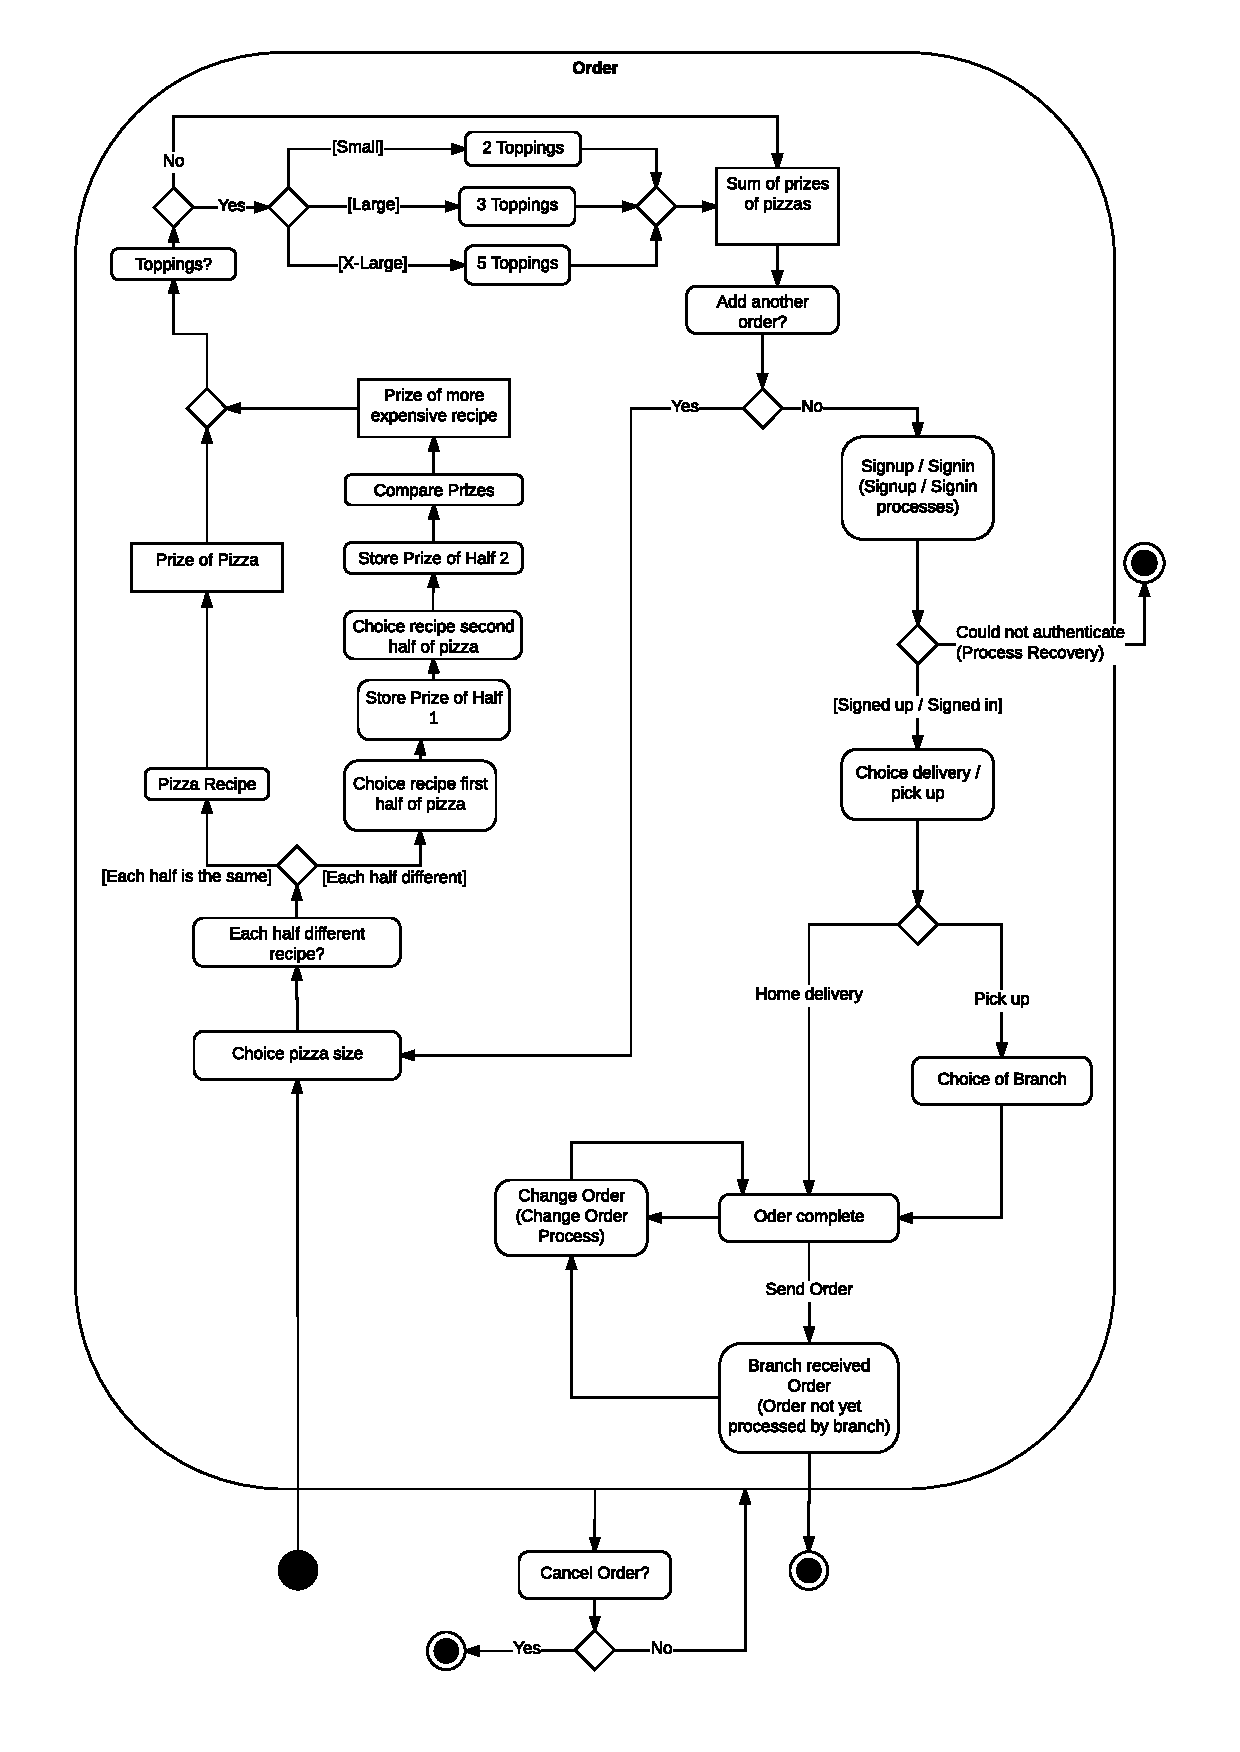
\includepdf[pages=-]{Activitydiagram.pdf}


%\begin{lstlisting}
%Put your code here.
%\end{lstlisting}



\end{document}
